\documentclass[a4paper,11pt]{article}
% Encodage et langue
\usepackage[utf8]{inputenc}
\usepackage[T1]{fontenc}
\usepackage[french]{babel}

% Polices et symboles mathématiques
\usepackage{amsfonts,amssymb,amsmath,mathrsfs,stmaryrd}

% Tableaux
\usepackage{boldline,multirow,tabularx,colortbl,diagbox,makecell,ltablex}

% Graphiques et couleurs
\usepackage{pgf,tikz,xcolor,pgfplots,pgfplotstable}
\usetikzlibrary{calc,positioning,shapes.geometric,shapes.symbols,shapes.misc,fit,shapes,arrows,arrows.meta}
\pgfplotsset{compat=1.18}

% Mise en page et style
\usepackage[top=2.5cm, bottom=2.5cm, left=2.25cm, right=2.25cm]{geometry}
\usepackage{setspace}
\usepackage{fancyhdr}
\usepackage{indentfirst}
\usepackage{adjustbox}
\usepackage{caption}
\usepackage{multicol}

% Hyperliens
\usepackage{hyperref}

% Diagrammes UML
\usepackage{plantuml}

% remarques et commentaires
\usepackage[colorinlistoftodos]{todonotes}



%==[DO NOT CHANGE ANYTHING HERE]====================
\newcommand{\addstudent}[3]{\small{#1} & \small{#2} & \small{\href{mailto:#3}{#3}}\\}
\newcommand{\addtutor}[2]{#1 & #2\\}
%==[DO NOT CHANGE ANYTHING BEFORE THIS LINE]====================

% Your PIR project title here
\def\projecttitle{
    Formats de fichiers 3D pour l'ingénierie de la construction
}

% Your keywords here
\def\varkeywords{
    Ingénierie collaborative pour le bâtiment; analyse des formats de fichiers, interopérabilité, formats 3D, disponibilité de l'information, ingénierie.
}

% Your names here
\def\students{
    \addstudent{Cyprien}{Pierre}{cyprien.pierre@uphf.fr}
    %\addstudent{Name}{SURNAME}{name.surname@mail.com}
    %\addstudent{Name}{SURNAME}{name.surname@mail.com}
}

% Your tutors here
\def\tutors{
    \addtutor{Alexis}{Heloir}
    %\addtutor{Name}{SURNAME}
}

\newcommand\tab[1][0.6cm]{\hspace*{#1}} %Create and define tab


%Chapter No Numbering but appears in TOC
\newcommand{\chapternn}[1]{\chapter*{#1}\addcontentsline{toc}{chapter}{#1}}
\newcommand{\sectionnn}[1]{\section*{#1}\addcontentsline{toc}{section}{#1}}
\newcommand{\subsectionnn}[1]{\subsection*{#1}\addcontentsline{toc}{subsection}{#1}}
\newcommand{\subsubsectionnn}[1]{\subsubsection*{#1}\addcontentsline{toc}{subsubsection}{#1}}

\newcolumntype{L}[1]{>{\raggedright\arraybackslash\hspace{0pt}}p{#1}}
\newcolumntype{R}[1]{>{\raggedleft\arraybackslash\hspace{0pt}}p{#1}}
\newcolumntype{C}[1]{>{\centering\arraybackslash\hspace{0pt}}p{#1}}

\renewcommand\thesection{\arabic{section}}
\renewcommand\thesubsection{\thesection.\arabic{subsection}}

\RequirePackage{fancyhdr}
\pagestyle{fancy}

%------- Do not append new commands after :

\hypersetup{	
    colorlinks  = false, % colorise les liens
    linkbordercolor = {1 1 1},
    breaklinks  = true, % permet le retour à la ligne dans les liens trop longs
    urlcolor    = blue, % couleur des hyperliens 
    linkcolor   = black,	% couleur des liens internes 
    citecolor   = black,	% couleur des références 
    pdftitle    = {Security assessment of connected objects in the Internet of Things : State of the art}, % informations apparaissant dans 
    pdfauthor   = {}, % les informations du document 
    pdfsubject  = {}	% sous Acrobat. 
}
\title{\vspace{1.5cm}Rapport de veille technologique \\ \vspace{0.25cm} \LARGE{\textbf{\projecttitle}}}
\author{}
\date{\today}
\RequirePackage{fancyhdr}
\pagestyle{fancy}
\renewcommand{\headrule}{}
\lhead{}
\chead{}
\rhead{}
\lfoot{\projecttitle}
\cfoot{}
\rfoot{\thepage}

\AtBeginDocument{\pagenumbering{gobble}
\thispagestyle{empty}

\pagenumbering{gobble}
\maketitle
\vspace{0.5cm}
\hrule
\vspace{1cm}

\noindent\begin{tikzpicture}[remember picture, overlay, shift={(current page.south west)}]
    %Images
    \node[anchor=north west] at (2,27.7) {
\includegraphics[height=1.225cm, keepaspectratio]{cover/meta/logo_insat.pdf}};
    \node[anchor=north west] at (2,26.25) {Département de Génie Civil};
    \node[anchor=north] at (21/2+1,27.7) {
\includegraphics[height=1.225cm, keepaspectratio]{cover/meta/univ.pdf}};
    %\node[anchor=north east] at (21-2,27.7) {
\includegraphics[height=1.225cm, keepaspectratio]{cover/meta/laas.jpg}};
    \node[anchor=north east] at (21-2,27.7) {
\includegraphics[height=1.225cm, keepaspectratio]{cover/meta/laas-light.png}};
\end{tikzpicture}

\begin{center}
    \textbf{Étudiants :}
    \vspace{0.25cm}
    
    \begin{tabular}{lll}
        \students
    \end{tabular}
\end{center}
\vspace{0.5cm}

\begin{center}
    \textbf{Tuteur :}
    \vspace{0.25cm}
    
    \begin{tabular}{lll}
        \tutors
    \end{tabular}
\end{center}\vspace{0.2cm}

\begin{center}
    \textbf{Keywords:}
    \varkeywords
\end{center}
\vspace{0.5cm}

\begin{center}
    \Large{\textbf{Résumé :}}
\end{center}
Ce rapport présente les formats de fichiers 3D utilisables dans le domaine de l'industrie de la construction. Il expose un ensemble de formats et les compare suivant les thématiques d'interopérabilité, de commissionnement, d'adoption par l'industrie et propose une analyse prospective quand à leurs usages futurs.

Le rapport expose que certains formats de fichiers sont à privilégier en rapport de l'objectif de l'utilisateur mais également quand à la pérennité du dit format.

\newpage
\pagestyle{fancy}
\lhead{}
\chead{}
\rhead{}
\lfoot{\projecttitle}
\cfoot{}
\rfoot{}
\doublespacing
\tableofcontents
\singlespacing
\newpage

\pagenumbering{arabic}
\pagestyle{fancy}
\lhead{}
\chead{}
\rhead{}
\lfoot{\projecttitle}
\cfoot{}
\rfoot{\thepage}


\newpage
\pagestyle{fancy}
\lhead{}
\chead{}
\rhead{}
\lfoot{\projecttitle}
\cfoot{}
\rfoot{}
\doublespacing
\listoffigures
\listoftables
\singlespacing
\newpage

\pagenumbering{arabic}
\pagestyle{fancy}
\lhead{}
\chead{}
\rhead{}
\lfoot{\projecttitle}
\cfoot{}
\rfoot{\thepage}}

\AtEndDocument{\input{cover/cover_out.tex}}

\begin{document}
    \sectionnn{Introduction}

Le temps du stylo Rotring et des planches à dessin n'est plus qu'un lointain souvenir dans l'univers de la construction. Depuis l'avènement de la conception assisté par ordinateur (CAO), Bureaux d'études, Maîtres d'ouvrages et Architectes se sont tournés vers les technologies de l'information pour gagner en rapidité et en qualité.

Cependant, l'industrie de la construction fait l'objet de nombreuses innovations ces dernières années. Des technologies issues d'autres secteurs industriels comme les industries manufacturières, le jeu vidéo ou encore les technologies de l'information viennent enrichir les outils à disposition des experts de la construction. 

Ces nouveaux apports à la filière viennent parfois bousculer des paradigmes de conception bien ancrés.

La modélisation 3D et les systèmes de Big Data ont permis l'avènement de la modélisation paramétrique et la réalisation de maquettes numériques de hautes précision, les modèles reposant sur l'intelligence artificielle générative accompagnent les études architecturales et la robotique comme l'impression 3D font leurs apparitions sur les chantiers.

L'ensemble de ces changements reposent sur un concept simple : l'information doit être partagée entre tous les acteurs et la collaboration est la clé de l'efficacité.

Pour atteindre cet objectif, de nombreux outils, standards et méthodologies ont été mise au point. Parmi eux, c'est le framework \textit{Virtual Design and Construction}\cite{brittanygielReturnInvestmentAnalysis2013} (VDC) accompagné des outils de \textit{Building Information Modeling}\cite{burcinbecerik-gerberPERCEIVEDVALUEBUILDING2010} (BIM) et le standard international, \textit{l'Industry Foundation Classes}\cite{yacinerezguiGOVERNANCEAPPROACHBIM2013} (IFC) qui ont été adoptés largement par la communauté.


Aujourd'hui, 12 ans après la percée de ces nouveaux paradigmes sur le territoire français, les promesses de collaboration et de simplifications initiales semblent pourtant être encore loin de la réalité.

Il n'existe sur le marché aucune plate-forme de conception offrant de la collaboration multi-curseur instantanée. Les technologies Cloud tendent à maintenir les paradigmes de travail en silos de données (travail isolé) et les plates-formes dites "collaboratives" n'offrent que peu voir pas de fonctionnalité d'ingénierie. 

Une des raisons pouvant justifier ces constats peut être que : seules les technologies du web peuvent permettre une collaboration efficace entre les différents corps d'état, mais ces technologies n'ont pas été pensées pour le domaine qui nous concerne.

C'est sur la base de cette réflexion que j'ai démarré mon étude des standards du web et de leurs rapprochements possibles avec le format IFC et les autres standards de l'ingénierie.

Ce rapport vient exposer les facultés offertes par un ensemble de formats de données 3D permettant le partage des informations géométriques des objets de la constructions tout en leur associant leurs données techniques. 

Ont été retenus uniquement les formats en sources ouvertes suivants : QIF, IFC, CityGML, USD et glTF.

Ce choix permettra de mieux exposer les enjeux liés à la sélection d'un format de fichier au dépens d'un autre selon l'objectif à atteindre. Un filtre préliminaire a été effectué afin ne pas surcharger ce rapport. Il conviendrait d'étudier chaque cas d'usage avec leurs formats de fichiers indépendamment. (e.g. la modélisation des espaces urbains via l'utilisation de CityGML, LandXML et autres.)

Cette restriction du domaine d'étude est également établie en considérant les contraintes d'interopérabilité. Ont donc étés écartés par défaut les formats de fichiers lorsqu'ils se trouvent :
\begin{itemize}
    \item être des formats propriétaires ou de spécification payante ;
    \item ne disposant pas d'un schéma standardisé ;
    \item ne pas être activement maintenu ;
    \item ne pas être largement adopté par l'industrie.
\end{itemize}

Seule exception faite pour le format QIF. Cette exception sera défendue plus tard dans le rapport.

\smallskip







\newpage

\section{Rapport d'analyse}

\subsection{Définition des besoins}

Les formats de fichiers 3D interviennent à diverses étapes d'un processus d'ingénierie de la construction.

Pour illustrer l'étude, considérons la réalisation d'un projet industriel à grande échelle consistant à distribuer de l'électricité à une zone d'activité exploitée par un acteur unique. 

Nous définissons ainsi les éléments suivants :
\begin{itemize}
    \item un site industriel avec des bâtiments existants, de la voirie et des réseaux,
    \item des bâtiments nouveaux (par exemple : des postes hautes tensions),
    \item des équipements (transformateurs, armoires électriques, cheminements...), 
    \item des composants (disjoncteurs, automates, bornes de raccordement...).
\end{itemize}

Cette première définition permet une identification claire des différents niveaux de détails, de macroscopique (le site) à microscopique (les composants).

Ensuite, il convient de se demander ce qui est attendu d'un format de fichier 3D dans un processus d'ingénierie. Les réponses peuvent être multiples. 

Voici la liste que je choisis de retenir pour notre étude :

\begin{itemize}
    \item réaliser un rendu 3D photo-réaliste du projet s'inscrivant dans le site existant,
    \item exécuter les travaux, comprenant l'installation des équipements,
    \item fabriquer les équipements,
    \item assurer le maintiens des informations durant la période d'exploitation et de maintenance.
\end{itemize}

Chaque format sera évalué en tenant compte de ces deux modes de catégorisation des besoins.

\newpage

\subsection{Arbitrage des formats}

L'univers de la modélisation 3D regorge de formats et de standards. Dans l'optique de réduire le champ d'étude, nous allons nous concentrer sur les formats qui sont libre et de source ouverte (FOSS), modifiables (not Flat), qui peuvent être utilisés pour l'ingénierie et dont le schéma de donnée peut être étendu.

Le tableau suivant illustre ce premier niveau d'arbitrage pour 20 formats de fichiers 3D, intégrant les formats les plus répandus sur le marché.

% Définitions des couleurs
\definecolor{mygreen}{RGB}{0, 255, 0}
\definecolor{myred}{RGB}{255, 0, 0}

% Commandes pour colorier les cellules selon les conditions
\newcommand{\fosscolor}[1]{\ifthenelse{\equal{#1}{Oui}}{\textcolor{mygreen}{#1}}{\textcolor{myred}{#1}}}
\newcommand{\flatcolor}[1]{\ifthenelse{\equal{#1}{Non}}{\textcolor{mygreen}{#1}}{\textcolor{myred}{#1}}}
\newcommand{\domainecolor}[1]{\ifthenelse{\equal{#1}{Impression 3D}}{\textcolor{myred}{#1}}{#1}}
\newcommand{\extensiblecolor}[1]{\ifthenelse{\equal{#1}{Oui}}{\textcolor{mygreen}{#1}}{\textcolor{myred}{#1}}}


\begin{table}[!h]
    \centering
    \caption{Tableau des formats de fichiers avec leurs caractéristiques}
    \renewcommand{\arraystretch}{1.5} 
    \begin{tabularx}{\textwidth}{|l|X|X|X|X|X|} 
        \hline
        \rowcolor{white!75!black} \textbf{Format} & \textbf{FOSS} & \textbf{Flat} & \textbf{Domaines d'utilisation} & \textbf{Extensible} \\
        \hline
        \textbf{QIF} & \fosscolor{Oui} & \flatcolor{Non} & \domainecolor{Qualité des données 3D} & \extensiblecolor{Oui} \\
        \hline
        \textbf{IFC} & \fosscolor{Oui} & \flatcolor{Non} & \domainecolor{Construction BIM} & \extensiblecolor{Oui} \\
        \hline
        \textbf{glTF} & \fosscolor{Oui} & \flatcolor{Non} & \domainecolor{Web, jeux vidéo} & \extensiblecolor{Oui} \\
        \hline
        \textbf{USD} & \fosscolor{Oui} & \flatcolor{Non} & \domainecolor{Animation 3D} & \extensiblecolor{Oui} \\
        \hline
        \textbf{CityGML} & \fosscolor{Oui} & \flatcolor{Non} & \domainecolor{Modélisation urbaine} & \extensiblecolor{Oui} \\
        \hline
        \textbf{OBJ} & \fosscolor{Oui} & \flatcolor{Oui} & \domainecolor{Modélisation 3D} & \extensiblecolor{Non} \\
        \hline
        \textbf{FBX} & \fosscolor{Non} & \flatcolor{Non} & \domainecolor{Animation 3D} & \extensiblecolor{Oui} \\
        \hline
        \textbf{IGES} & \fosscolor{Oui} & \flatcolor{Oui} & \domainecolor{CAO, échange de données} & \extensiblecolor{Non} \\
        \hline
        \textbf{STEP} & \fosscolor{Oui} & \flatcolor{Non} & \domainecolor{CAO, échange de données} & \extensiblecolor{Oui} \\
        \hline
        \textbf{IPT} & \fosscolor{Non} & \flatcolor{Non} & \domainecolor{CAO Autodesk} & \extensiblecolor{Non} \\
        \hline
        \textbf{IAM} & \fosscolor{Non} & \flatcolor{Non} & \domainecolor{CAO Siemens} & \extensiblecolor{Non} \\
        \hline
        \textbf{SLD} & \fosscolor{Non} & \flatcolor{Non} & \domainecolor{CAO Dassault Systèmes} & \extensiblecolor{Non} \\
        \hline
        \textbf{JT} & \fosscolor{Non} & \flatcolor{Non} & \domainecolor{Visualisation 3D} & \extensiblecolor{Non} \\
        \hline
        \textbf{AMF} & \fosscolor{Oui} & \flatcolor{Non} & \domainecolor{Impression 3D} & \extensiblecolor{Oui} \\
        \hline
        \textbf{STL} & \fosscolor{Oui} & \flatcolor{Oui} & \domainecolor{Impression 3D} & \extensiblecolor{Non} \\
        \hline
        \textbf{X3D} & \fosscolor{Oui} & \flatcolor{Non} & \domainecolor{Web 3D} & \extensiblecolor{Oui} \\
        \hline
        \textbf{3DS} & \fosscolor{Non} & \flatcolor{Non} & \domainecolor{Modélisation 3D} & \extensiblecolor{Non} \\
        \hline
        \textbf{3MF} & \fosscolor{Oui} & \flatcolor{Non} & \domainecolor{Impression 3D} & \extensiblecolor{Oui} \\
        \hline
        \textbf{DAE} & \fosscolor{Oui} & \flatcolor{Non} & \domainecolor{Animation 3D} & \extensiblecolor{Oui} \\
        \hline
        \textbf{DWG} & \fosscolor{Non} & \flatcolor{Non} & \domainecolor{CAO AutoCAD} & \extensiblecolor{Non} \\
        \hline
    \end{tabularx}
\end{table}

Dans un second temps, je choisis délibérément d'écarter le format STEP de l'étude car il est à l'origine de la création des formats QIF et IFC. Il est alors plus intéressant d'analyser ce que ces deux autres formats ont à proposer au regard de leurs domaines d'utilisations respectifs.

Également, n'ayant trouvé que peut voir aucun travaux permettant de rapprocher efficacement les formats DAE et X3D de l'ingénierie de la construction, ils sont donc écartés.

\newpage

\subsection{Présentation des formats}


Avant de commencer l'étude de cas, découvrons les formats de fichiers retenus.

\begin{figure}[!h]
    \centering
    
\includegraphics[width=1\linewidth]{imports/3DFiles_Logos.pdf}
    \caption{Logos des formats}
    \label{fig:enter-label}
\end{figure}

Le tableau suivant donne des informations générales sur ces formats :

\begin{table}[!h]
    \centering
    \caption{Informations générales des formats de fichiers}
    \renewcommand{\arraystretch}{1.5} 
    \begin{tabularx}{\textwidth}{|l|X|X|X|X|X|} 
        \hline
        \rowcolor{white!75!black} \textbf{} & \textbf{QIF\cite{githubGitHubQualityInformationFrameworkqifcommunity}} & \textbf{IFC\cite{githubGitHubBuildingSMARTIFC43xdevelopment}} & \textbf{CityGML\cite{githubGitHubOpengeospatialCityGML30CM}} & \textbf{USD\cite{githubGitHubPixarAnimationStudiosOpenUSD}} & \textbf{glTF\cite{githubGitHubKhronosGroupglTF}}\\
        \hline
        \textbf{Nom complet} & Quality Information Framework & Industry Foundation Classes & City Geography Markup Language & Universal Scene Description & Graphics Language Transmission Format\\
        \hline
        \textbf{Développé par} & Digital Metrology Standards Consortium & building SMART International & Open Geospatial Consortium & Alliance for Open USD & Khronos Group \\
        \hline
        \textbf{Normalisation} & ISO 23952 & ISO 16739 & série ISO 19100 & Néant & ISO 12113 \\
        \hline
        \textbf{Licence} & BSL-1.0 & CC BY-ND 4.0 & MIT & Apache 2.0 Modifiée &  Multiples \\
        \hline
    \end{tabularx}
\end{table}

L'ensemble de ces formats sont gratuits et de sources ouvertes.

\newpage

\subsubsection{QIF}
Ce format de fichier vise à étendre les capacités des formats de CAO utilisés dans les industries manufacturières. Il intègre 6 schémas de données standardisés permettant notamment la sauvegarde des informations de métrologie, les bonnes pratiques et les comportements des éléments.
\begin{quote}
    The goal of the QIF specification is to facilitate interoperability of manufacturing quality data between system software components. \cite{QualityInformationFramework2018}
\end{quote}
Il est principalement destiné à être utilisé au travers des solutions de type Product Lifecycle Management (PLM) et de Manufacturing Execution System (MES).

\subsubsection{IFC}
Ce format tend à offrir à l'ensemble du secteur de la construction une définition commune des objets utilisés dans cette industrie. Le format IFC ressemble pour la construction à ce qu'est le PDF pour la documentation.\cite{ffbatimentQuestceQuun}
\begin{quote}
    Les IFC sont développés à partir de 1996 par buildingSMART International afin de favoriser l’interopérabilité dans le secteur du Bâtiment, et depuis peu une intégration des Infrastructures est en cours. \cite{picinbonoIFCPratique2018}
\end{quote}
Il est principalement utilisé pour transmettre des données géométriques et alphanumériques sur des ouvrages entre les corps d'état et les différentes spécialités de la construction.

\subsubsection{CityGML}
CityGML propose d'enregistrer, dans une source unique, toutes les informations relatives à une ville. Cela comprend, entre autres, la planification urbaine, la conception architecturale, la simulation environnementale, la navigation des véhicules et des piétons.
\begin{quote}
    The CityGML Conceptual Model Standard defines a common semantic information model for the representation of 3D urban objects that can be shared over different applications. \cite{kolbeOGCCityGeography2021}
\end{quote}
Il est principalement utilisé dans les solutions de Geographic Information System (GIS) et de City Information Modeling (CIM).

\subsubsection{USD}
L'USD permet de regrouper dans un fichier unique l'ensemble des données et ressources nécessaires à la génération d'un environnement de très haute qualité graphique. 
\begin{quote}
    USD is a high-performance extensible software platform for collaboratively constructing animated 3D scenes, designed to meet the needs of large-scale film and visual effects production. \cite{noauthor_usd_nodate}
\end{quote}
Il est utilisé par de nombreux logiciels de modélisation destinés à l'industrie du cinéma et des jeux vidéo.

\subsubsection{glTF}
Ce standard du Web 2.0 affirme clairement être l'égal du JPEG en matière de format 3D. Il se veut léger et compatible nativement avec les navigateurs web comme l'explique cette citation tirée du site du consortium Chronos :\cite{khronosGlTFRuntime}
\begin{quote}
   glTF is an open interoperable 3D asset ‘transmission’ format that is compact, and efficient to process and render at runtime. glTF 2.0 is designed to be vendor- and runtime-neutral, usable by a wide variety of native and web-based engines and applications regardless of underlying platforms and 3D graphics APIs.. \cite{GlTFSpecification2021}
\end{quote}    
glTF est utilisé aussi bien par des logiciels de modélisations de tout domaine que par des applications web.

\newpage

\subsection{Sémantique}
L'analyse de la sémantique supportée par chaque format est une opération cruciale lorsque l'on cherche à comprendre les capacité du dit format. C'est également un exercice long et fastidieux qu'il aurait été bien difficile à réaliser pour la présente revue. 

Le tableau suivant expose donc quelques éléments d'ordres généraux et leurs prises en charges par notre sélection de formats.

\begin{table}[!h]
    \centering
    \caption{Analyse sémantique macroscopique des formats}
    \renewcommand{\arraystretch}{1.5} 
    \begin{tabularx}{\textwidth}{|l|X|X|X|X|X|} 
        \hline
        \rowcolor{white!75!black} \textbf{} & \textbf{QIF} & \textbf{IFC} & \textbf{CityGML} & \textbf{USD} & \textbf{glTF}\\
        \hline
        \textbf{Format de donnée} & XML & EXPRESS & XML, JSON avec CityJSON & BINAIRE & JSON \\
        \hline
        \textbf{Type d'objet 3D} & STEP (BREP) & STEP (BREP) & BREP & BINAIRE & MESHES \\
        \hline
        \textbf{Extensions} & .qif & .ifc ; .ifcxml ; .ifczip & .gml ; .xml & .usda ; .usdc ; .usdz  & .gltf ; .glb  \\
        \hline
        \textbf{Matériaux} & \textcolor{orange}{*\footnotemark{}} & \textcolor{green}{Oui} & \textcolor{green}{Oui} & \textcolor{green}{Oui} & \textcolor{green}{Oui} \\
        \hline
        \textbf{Textures} & \textcolor{orange}{*\footnotemark[\value{footnote}]} & \textcolor{green}{Oui} & \textcolor{green}{Oui} & \textcolor{green}{Oui} & \textcolor{green}{Oui} \\
        \hline
        \textbf{Couleurs} & \textcolor{orange}{*\footnotemark[\value{footnote}]} & \textcolor{green}{Oui} & \textcolor{green}{Oui} & \textcolor{green}{Oui} & \textcolor{green}{Oui} \\
        \hline
        \textbf{Shaders} & \textcolor{orange}{*\footnotemark[\value{footnote}]} & \textcolor{red}{Non} & \textcolor{red}{Non} & \textcolor{green}{Oui} & \textcolor{green}{Oui} \\
        \hline
        \textbf{Tolérances} &  \textcolor{green}{Oui} & \textcolor{green}{Oui} & \textcolor{red}{Non} & \textcolor{red}{Non} & \textcolor{red}{Non} \\
        \hline
        \textbf{Niveau de détail adaptatif} & \textcolor{red}{Non} & \textcolor{red}{Non} & \textcolor{green}{Oui} & \textcolor{green}{Oui} & \textcolor{green}{Oui} \\
        \hline
        \textbf{Symboles et annotations} & \textcolor{orange}{*\footnotemark[\value{footnote}]} & \textcolor{green}{Oui} & \textcolor{green}{Oui} & \textcolor{green}{Oui} & \textcolor{red}{Non} \\
        \hline
        \textbf{Scripts et Automatisations} & \textcolor{orange}{*\footnotemark[\value{footnote}]} & \textcolor{red}{Non} & \textcolor{red}{Non} & \textcolor{green}{Oui} & \textcolor{red}{Non} \\
        \hline
    \end{tabularx}
\end{table}

Il faut bien noter ici que chacun de ces formats a été conçu avec un objectif différent des autres. Les ressemblances et rapprochements sémantiques n'ont d'autres intérêts que d'identifier les connexion possibles entre chacun de ces fichiers lorsqu'ils sont utilisés dans des contextes différents mais nécessitant une interaction (e.g déplacer un bâtiment en changeant le géoréférencement d'un IFC et mettre à jour son jumeau présent dans le CityGML).

\footnotetext{Dépend du format de l'asset 3D initial. Est généralement utilisé le format STEP qui, dans la liste, ne supporte pas les shaders.}

\newpage

\subsection{Cas d'usages}
Avant de pouvoir identifier précisément les formats les plus adaptés aux usages, commençons par définir ces derniers. Le diagramme suivant expose une vue macroscopique des cas d'usages en fonction du type d'acteur concerné.

\begin{figure}[!h]
    \centering
    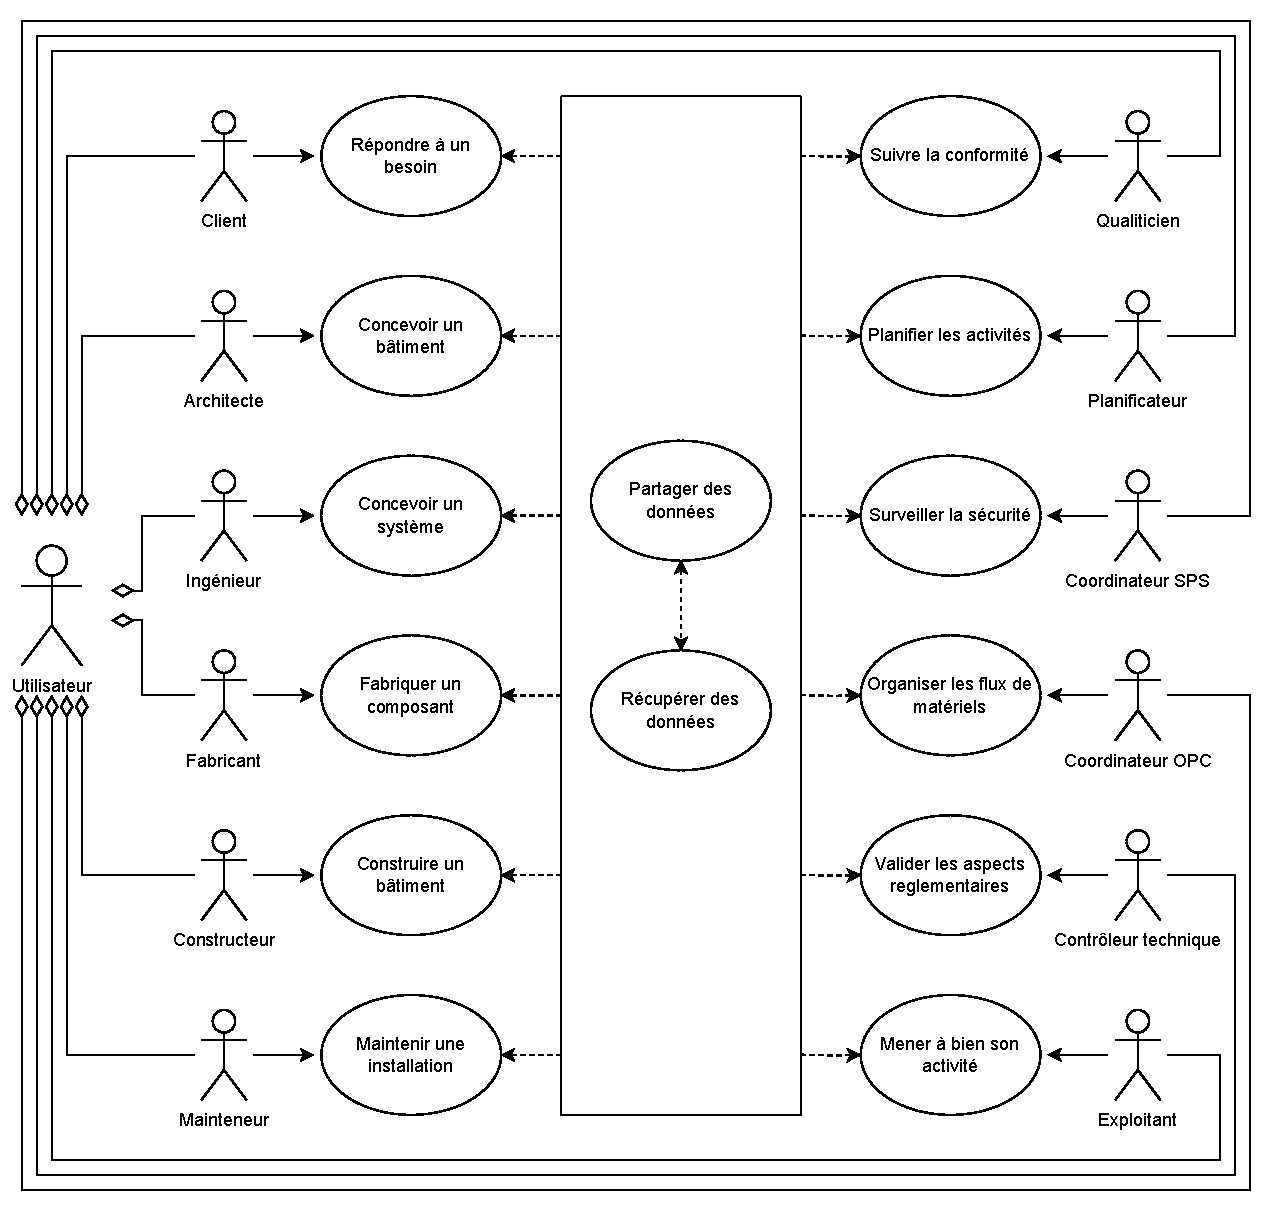
\includegraphics[width=1\linewidth]{imports/3DFiles_UseCase.pdf}
    \caption{Diagramme de cas d'usage - Partage d'information selon l'acteur concerné}
    \label{fig:enter-label}
\end{figure}

Chaque format 3D semble permettre, d'une façon ou d'une autre, de répondre à chacun de ces cas d'usage :
\begin{itemize}
    \item L'USD peut aider le constructeur à sélectionner la bonne teinte pour le ravalement de façade,
    \item le QIF peut aider dans la conception d'un système
    \item etc.
\end{itemize}
\newpage
Cependant, en regardant les catégories d'outils utilisés dans l'univers de la construction (du fabricant à l'exploitant), nous pouvons réaliser un nuage plus représentatif des environnements dans lesquels chaque format serait plus appropriés que ces comparses.

Le tableau suivante expose une matrice de sélection du format de fichier au regard de l'objectif d'ingénierie du bâtiment.

\begin{table}[!h]
    \centering
    \caption{Matrice de sélection du format de fichier}
    \renewcommand{\arraystretch}{1.5} 
    \begin{tabularx}{\textwidth}{|l|X|X|X|X|X|} 
        \hline
        \rowcolor{white!75!black} \textbf{} & \textbf{QIF} & \textbf{IFC} & \textbf{CityGML} & \textbf{USD} & \textbf{glTF}\\
        \hline
        \textbf{Computer Aided Design} & X & X & X &  & X \\
        \hline
        \textbf{Computer Aided Manufacturing} & X &  &  &  &  \\
        \hline
        \textbf{Computer Aided Inspection} & X &  &  &  &  \\
        \hline
        \textbf{Computer Aided Engineering} & X & X & X &  &  \\
        \hline
        \textbf{Augmented Reality} &  & X & X &  & X \\
        \hline
        \textbf{Mixed Reality} &  & X & X &  & X \\
        \hline        
        \textbf{Virtual Reality} &  &  &  & X & X \\
        \hline
    \end{tabularx}
\end{table}

Si nous reprenons notre contexte : 
\begin{quote}
    réalisation d'un projet industriel à grande échelle consistant à distribuer de l'électricité à une zone d'activité exploitée par un acteur unique.
\end{quote}

Nous pouvons identifier la répartition de l'utilisation des formats de la façon suivante :
\begin{itemize}
    \item QIF : Un fichier .qif porte les informations d'un élément (e.g. un transformateur HT). Il est édité par le fabricant et est transmis au concepteur qui en utilisera les données pour vérifier ses notes de calculs. Le fabricant utilisera également les informations pour fabriquer son équipement dont les assemblages d'éléments, ces derniers étant également au format QIF. 
    \item IFC : Le concepteur implante dans une maquette numérique l'ensemble des éléments nécessaires à la mise en oeuvre de son marché. Il en retire des nomenclatures et plans d'implantations.
    \item CityGML : L'architecte réalise les compositions architecturales et l'aménagement du site.
    \item USD : L'architecte réalise une vidéo d'immersion dans l'ouvrage pour présenter le projet au client.
    \item glTF : L'installateur, comme le mainteneur, peut visualiser en réalité mixte comme augmentée les installations à mettre en oeuvre ou à maintenir.
\end{itemize}

L'exploitant du projet dispose de plusieurs niveaux de granularité et d'outils complémentaires lui permettant de faciliter l'ensemble de ses activités (accès aux documentations techniques, hypervision, etc.)

\newpage

\subsection{Interopérabilité}

La notion d'interopérabilité peut être confuse. Le site internet fr.wikitionary.org donne la définition suivante :

\begin{quote}
    Capacité que possède un produit ou un système, dont les interfaces sont intégralement connues, à fonctionner avec d’autres produits ou systèmes existants ou futurs et ce sans restriction d’accès ou de mise en œuvre. 
    \cite{wiktionaryInteroprabilitWiktionnaire}
\end{quote}

Cette définition donne, pour notre cas d'étude, les prérogatives suivantes :

\begin{enumerate}
    \item Les formats de fichiers, à périmètre donné, doivent pouvoir fonctionner ensemble. C'est-à-dire qu'ils aient la capacité d'être imbriqués ou étendus les uns par rapport aux autres.
    \item Leurs utilisations et prise en charge doivent être rendu possible par une ouverture totale de leurs schémas de constructions. C'est-à-dire que tout organisme développant une solution informatique doit pouvoir accéder librement au code source et aux normes permettant la manipulation des dits formats.
\end{enumerate}

\subsubsection{Liaison inter-formats}

La figure suivante illustre l'interopérabilité entre les formats de fichiers et vient donner un aperçu de la réponse au point n°1 :

\begin{figure}[!h]
    \centering
    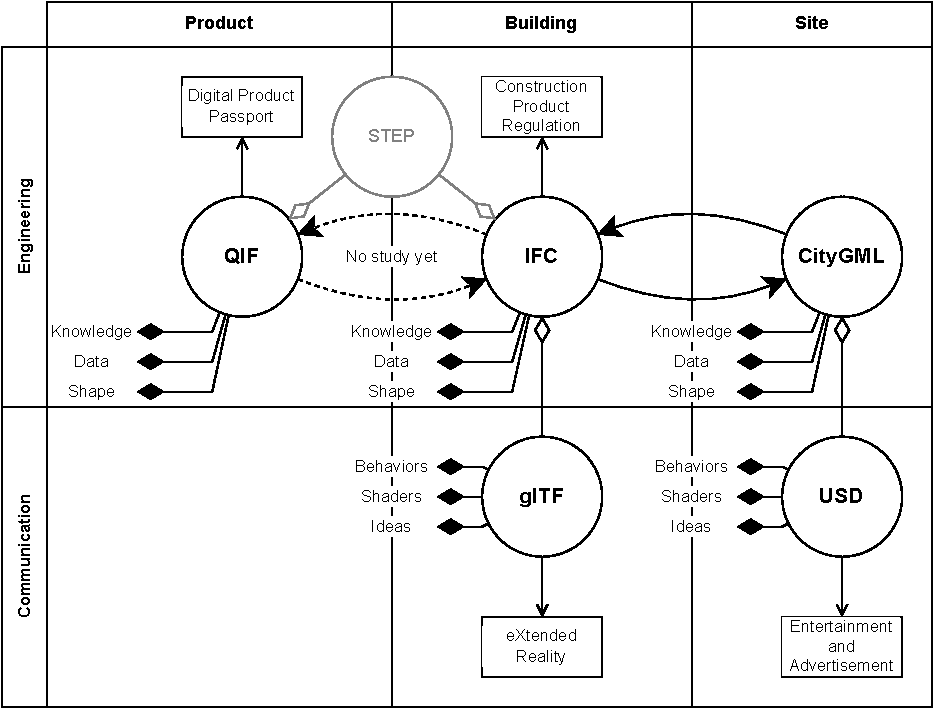
\includegraphics[width=1\linewidth]{imports/3DFiles_Intrication.pdf}
    \caption{Interaction des formats de fichiers}
    \label{fig:enter-label}
\end{figure}

\subsubsection{Prise en charge par les logiciels}

Pour offrir un aperçu de l'atteinte de l'objectif décrit au point n°2, il faut s'intéresser à la prise en charge de ces formats par les outils favoris utilisés par les professionnels de la construction. Le tableau suivant représente une matrice de prose en charge. Les logiciels ont été choisis arbitrairement et la liste est non exhaustive. Cet exercice est donc proposé à titre d'illustration de la démarche à adopter pour une étude plus large sur ce sujet.

\begin{table}[!h]
    \centering
    \caption{Prise en charge des formats par quelques logiciels}
    \renewcommand{\arraystretch}{1.25} 
    \small
    \begin{tabularx}{\textwidth}{|l|X|X|X|X|X|} 
        \hline
        \rowcolor{white!75!black} \textbf{} & \textbf{QIF} & \textbf{IFC} & \textbf{CityGML} & \textbf{USD} & \textbf{glTF}\\
        \hline
        \textbf{AutoCAD et associés} & Non & Natif & Map 3D, Civil 3D & Non & Non \\
        \hline
        \textbf{Revit} & Non & Natif & Non & Plugin\cite{prototechsolutionsCustomPlugins} & Plugin\cite{prototechsolutionsCustomPlugins} \\
        \hline
        \textbf{Inventor} & Export & Export & Non & Plugin\cite{prototechsolutionsCustomPlugins2} & Plugin\cite{prototechsolutionsCustomPlugins2} \\
        \hline
        \textbf{ArchiCAD} & Non & Natif & Non & Non & Non \\
        \hline
        \textbf{Blender} & Non & BlenderBIM & Non & Natif & Natif \\
        \hline
        \textbf{Solidworks} & Plugin pour l'export\cite{capvidiaExportNeutral} & Natif & Non & Non & Natif \\
        \hline
        \textbf{ArcGIS} & Non & Indoors Pro, Indoors Maps & CityEngine & Natif & Natif \\
        \hline
        \textbf{QGIS} & Non & Non & 3DCityDB Tools & Non & Natif \\
        \hline
    \end{tabularx}
\end{table}

\subsubsection{Web application}

Le portage du format IFC est théoriquement possible mais très compliqué. \cite{buildingsmartIfcOWLBuildingSMART,sciencedirectEXPRESSConstruction}
Le format glTF est conçu spécifiquement pour un usage web et une prise en charge par la librairie WebGL. \cite{githubGlTFTutorialsgltfTutorialgltfTutorial_001_IntroductionmdMain}
Le format CityGML pourrait être utilisé pour exposer des modèles de villes à travers des navigateurs web \cite{el-mekawyIntegratingBIMGIS2010,prandi3DWebVisualization2015} mais, a part quelques proof-of-concept, aucune réalisation à grande échelle ne semble avoir été réalisée à ce jour.
Les formats QIF et USD ne possède pas de documentation concernant leurs portage sur le web. Ces formats étant destinés à contenir un très grand nombre de donnée, il est concevable qu'ils ne soient pas pertinents dans un contexte web. 

\subsubsection{Contrôle et vérification}

Les fichiers servant de réceptacles d'information et permettant leur diffusion, il est important de l'assurer qu'ils répondent effectivement à leur propre standard. Pour cela, chaque format dispose de ses propres outils de validation. 
Le tableau suivant expose sommairement les technologies employées pour vérifier chaque format :

\begin{table}[!h]
    \centering
    \caption{Technologie de validation des schémas de données}
    \renewcommand{\arraystretch}{1.5} 
    \small
    \begin{tabularx}{\textwidth}{|l|X|X|X|X|X|} 
        \hline
        \rowcolor{white!75!black} \textbf{} & \textbf{QIF} & \textbf{IFC} & \textbf{CityGML} & \textbf{USD} & \textbf{glTF}\\
        \hline
        \textbf{Validation} & XSLT & IDS & XSLT & Outils natifs USD & Outils tiers (e.g. JSON-Schema) \\
        \hline
    \end{tabularx}
\end{table}

\newpage

\subsection{Commissionnement}

Le commissionnement est défini tel que :
\begin{quote}
    l’approche méthodique visant à garantir que tous les éléments opérationnels d’un projet – depuis la planification et la conception jusqu’à la construction, la mise en œuvre ou l’installation proprement dite – fonctionnent comme ils le devraient. Il vise à inspecter, documenter et vérifier que l’avancement d’un projet est conforme aux exigences et aux spécifications du propriétaire du projet. En outre, la mise en service permet de corriger de manière proactive tout oubli dans les projets, évitant ainsi des modifications coûteuses par la suite.\cite{safetycultureCommissionnementDfinition}
\end{quote}

Aussi, la disponibilité et la pérennité des informations durant les phases de conception et de réalisation est primordiale. De plus, avec les enjeux du décret BACs et la montée en puissance des systèmes de GTB et de GMAO, ces prérogatives sont maintenues durant toute la vie d'un ouvrage. 

\subsubsection{Pérennité du format de fichier}

Dans le tableau suivant, sont recensés des données relatives à l'activité des dépôts de chacun des formats. 
Ces données ont été extraites depuis le site web \href{https://ossinsight.io}{ossinsight.io} via l'assistant "GitHub Data Explorer" utilisant le modèle d'intelligence artificielle "Chat2Query" de TiDB Cloud.

Ce modèle rédige des requêtes SQL sur la base d'une demande en langage naturel.

Voici le prompt utilisé : 

\begin{quote}
    \textit{Count the number of : Stars, Commits, Issues, Forks, PR Creators, Collaborators, add the Language and the date of last commit}
\end{quote}

Les données étant agrégées depuis une source externe à GitHub, elles peuvent ne pas correspondre exactement. J'ai remarqué seulement de très faibles écarts entre les données disponibles sur GitHub et celles fournies par Ossinsight (écart < 1\%). Seul le nombre de collaborateurs pour le format CityGML n'a pas été retrouvé par l'outil, cet indicateur portant à confusion avec "PR Creators" je l'ai écarté de l'étude.
Le langage d'implémentation n'a été que rarement fournis, je l'ai donc retiré de la synthèse.

\begin{table}[!h]
    \centering
    \caption{Synthèse des résultats des requêtes par format}
    \renewcommand{\arraystretch}{1.5} 
    \begin{tabularx}{\textwidth}{|l|X|X|X|X|X|} 
        \hline
        \rowcolor{white!75!black} \textbf{} & \textbf{QIF\footnote{https://ossinsight.io/analyze/QualityInformationFramework/qif-community}} & \textbf{IFC\footnote{https://ossinsight.io/analyze/buildingSMART/IFC4.3.x-development}} & \textbf{CityGML\footnote{https://ossinsight.io/analyze/opengeospatial/CityGML-3.0CM}} & \textbf{USD\footnote{https://ossinsight.io/analyze/PixarAnimationStudios/OpenUSD}} & \textbf{glTF\footnote{https://ossinsight.io/analyze/KhronosGroup/glTF}}\\
        \hline
        \textbf{Stars} & 28 & 145 & 83 & 5595 & 871 \\
        \hline
        \textbf{Commit} & 38 & 1633 & 150 & 11754 & 2255 \\
        \hline
        \textbf{Issues} & 35 & 3198 & 135 & 1666 & 1232 \\
        \hline
        \textbf{Forks} & 18 & 80 & 15 & 1138 & 1330 \\
        \hline
        \textbf{Pull Request Creators} & 1 & 35 & 2 & 195 & 196 \\
        \hline
        \textbf{Last commit date} & 2024-03-14 & 2024-05-27 & 2023-09-03 & 2024-05-31 & 2024-05-31 \\
        \hline
    \end{tabularx}
\end{table}

L'analyse de chaque indicateur permet d'obtenir une bonne approximation du cycle de vie des projets, allant de l'intérêt communautaire à l'implication des développeurs.

\newpage 

\textbf{Nombre d'étoiles :}
Le nombre d'étoiles permet, entre autres, d'illustrer l'intérêt et l'appréciation d'un projet.
Le graphique suivant reflète une très forte appréciation du format USD par la communauté avec 5 595 étoiles.
Le format glTF est également apprécié, il faut rester prudent à l'égard du score proposé ici puisque ce format est scindé en plusieurs dépôts adaptés aux besoins des utilisateurs.
Le format QIF n'étant que faiblement plébiscité, il ne possède que très peu d'étoiles.

\begin{figure}[!h]
    \centering
    \begin{tikzpicture}
        \begin{axis}[
            ybar,
            symbolic x coords={QIF, IFC, CityGML, USD, glTF},
            xtick=data,
            nodes near coords,
            ymin=0,
            xticklabel style={rotate=45, anchor=east},
            bar width=15pt,
            enlarge x limits={abs=0.75cm},
        ]
        \addplot coordinates {(QIF, 28) (IFC, 145) (CityGML, 83) (USD, 5595) (glTF, 871)};
        \end{axis}
    \end{tikzpicture}
    \caption{Nombre d'étoiles par format}
    \label{fig:mon_graphique}
\end{figure}

\textbf{Nombre de Commits}
Cet indicateur est un compteur du nombre de modifications apporté à un projet depuis sa création. Il permet d'évaluer notamment l'investissement de ses développeurs.
Ici encore, le format USD est loin devant ses concurrents. Les formats IFC et glTF sont également très actifs. 

\begin{figure}[!h]
    \centering
    \begin{tikzpicture}
        \begin{axis}[
            ybar,
            symbolic x coords={QIF, IFC, CityGML, USD, glTF},
            xtick=data,
            nodes near coords,
            ymin=0,
            xticklabel style={rotate=45, anchor=east},
            bar width=15pt,
            enlarge x limits={abs=0.75cm},
        ]
        \addplot coordinates {(QIF, 38) (IFC, 1633) (CityGML, 150) (USD, 11754) (glTF, 2255)};
        \end{axis}
    \end{tikzpicture}
    \caption{Nombre de commits par format}
    \label{fig:mon_graphique}
\end{figure}

\textbf{Nombre d'Issues}
Cette donnée permet de suivre l'état de santé d'un projet. Par extrapolation, il indique également l'intérêt de la communauté. Tout utilisateur d'un projet peut ouvrir une issue pour rapporter un bogue ou soumettre une évolution.
Cette fois, c'est le format IFC qui sort du lot avec 3 198 issues au compteur. Ce format de fichier faisant l'œuvre d'évolutions permanentes depuis son introduction, et au regard de sa volonté d'interopérabilité, il est assez normal que de nombreuses issues soient ouvertes. Un meilleur compteur ici serait de suivre le nombre d'issue ouverte et clôturée sur une période.
Les formats USD et glTF sont aussi très actifs sur ce plan.

\begin{figure}[!h]
    \centering
    \begin{tikzpicture}
        \begin{axis}[
            ybar,
            symbolic x coords={QIF, IFC, CityGML, USD, glTF},
            xtick=data,
            nodes near coords,
            ymin=0,
            xticklabel style={rotate=45, anchor=east},
            bar width=15pt,
            enlarge x limits={abs=0.75cm},
        ]
        \addplot coordinates {(QIF, 35) (IFC, 3198) (CityGML, 135) (USD, 1666) (glTF, 1232)};
        \end{axis}
    \end{tikzpicture}
    \caption{Nombre d'issue par format}
    \label{fig:mon_graphique}
\end{figure}

\textbf{Nombre de Forks}
Cette information est probablement la plus intéressante. Elle est le reflet immédiat de l'utilisation d'un projet par la communauté de développeur. Plus le nombre de fork est grand, plus il est probable que le projet source fasse consensus. 
Cette fois, et sans grande surprise, c'est le format glTF (un des standards du web) qui gagne la course, avec l'USD est très proche derrière. 
Enfin, la quasi-équivalence entre les formats QIF et CityGML est intéressante. Bien que QIF soit fortement méconnu et peu déployé, il obtient un meilleur ratio de fork par étoile (64\% contre 18\% pour le CityGML). Cela laisse à penser que ce format de donnée suscite l'intérêt des personnes le découvrant et qu'une meilleure exposition pourrait lui être bénéfique à moyen et long terme.

\begin{figure}[!h]
    \centering
    \begin{tikzpicture}
        \begin{axis}[
            ybar,
            symbolic x coords={QIF, IFC, CityGML, USD, glTF},
            xtick=data,
            nodes near coords,
            ymin=0,
            xticklabel style={rotate=45, anchor=east},
            bar width=15pt,
            enlarge x limits={abs=0.75cm},
        ]
        \addplot coordinates {(QIF, 18) (IFC, 80) (CityGML, 15) (USD, 1138) (glTF, 1330)};
        \end{axis}
    \end{tikzpicture}
    \caption{Nombre de forks par format}
    \label{fig:mon_graphique}
\end{figure}

\textbf{Nombre de créateur de Pull Request}
Cet indicateur reflète le nombre de personnes autorisées à proposer des modifications de code.
Nous remarquons que les formats USD et glTF sont maintenus par le même volume de développeur. 
Ici, il est intéressant de voir que QIF et CityGML sont maintenus que par respectivement 1 et 2 personnes. Cela peut poser un problème de partage de responsabilité et de longévité. Il serait intéressant pour ces projets d'étendre le maintien de leur base de développement à d'autres membres de leurs organisations.

\begin{figure}[!h]
    \centering
    \begin{tikzpicture}
        \begin{axis}[
            ybar,
            symbolic x coords={QIF, IFC, CityGML, USD, glTF},
            xtick=data,
            nodes near coords,
            ymin=0,
            xticklabel style={rotate=45, anchor=east},
            bar width=15pt,
            enlarge x limits={abs=0.75cm},
        ]
        \addplot coordinates {(QIF, 1) (IFC, 35) (CityGML, 2) (USD, 195) (glTF, 196)};
        \end{axis}
    \end{tikzpicture}
    \caption{Nombre de pull request par format}
    \label{fig:mon_graphique}
\end{figure}

\subsubsection{Cadre normatif}

La loi européenne dénommée Ecodesign for Sustainable Products Regulation (ESPR), défini un cadre quant au respect des enjeux environnementaux des produits. 
Elle introduit également le terme de passeport numérique de produit :

\begin{quote}
    The new “Digital Product Passport” will provide information about products’ environmental sustainability. This information will be easily accessible by scanning a data carrier and it will include attributes such as the durability and reparability, the recycled content or the availability of spare parts of a product. \cite{europaEcodesignSustainable}
\end{quote}

Le champ d'application est aujourd'hui restreint mais tend à s'élargir notamment aux produits de la construction :

\begin{quote}
    Le passeport numérique des produits sera exigé pour l’ensemble des produits couverts par le règlement ESPR ainsi que d’autres règlements comme celui de la construction (CPR) ou celui des batteries (EVs batteries). \cite{PasseportNumeriqueProduits}
\end{quote}

Les normes de performance environnementales et les labels de performance, y compris en qualité de l'air, entraînent un besoin grandissant d'information au sujet des éléments constitutif de toute construction. 
Les sources de données sont très variées et difficilement rapprochables sans l'usage d'outils spécifiques (e.g. IZUBA Pleiades avec les modules ACV et Indalo). 

Les contraintes de traçabilités demandés dans certaines industries (santé, aérospatial, nucléaire, défense...) sont également des contraintes significatives rencontrées par les constructeurs.

L'intégration de ces données au sein même des assets 3D utilisés pour réaliser la construction d'un ouvrage offrirait une grande aisance aux constructeurs pour justifier leurs respects des normes et exigences ainsi qu'aux exploitants dans leurs opérations de gestion, exploitation et maintenance. 

A ce sujet, j'estime que le format QIF, de par sa nature, est un excellent candidat dans la réalisation de cette tâche. Le format IFC offre également quelques possibilités concernant les ouvrages de génie civil.

\newpage

%\input{content/2.part.tex}
%\newpage

%\input{content/3.part.tex}
%\newpage

\section{Conclusion}

L'étude expose que les formats QIF, IFC et CityGML sont d'excellents containers d'informations pour l'ingénierie de la construction. A contrario, les formats USD et glTF offrent de meilleurs perspectives dans les domaines de la réalité étendue et des environnements immersifs. 

Les graphiques suivants résument, pour chaque format étudié, les 5 points d'analyse que nous avons parcourus : les fonctionnalités techniques offertes par le standard, son adoption dans l'industrie, la complexité de son schéma, la pérennité et la stabilité présumée à date. 

\begin{figure}[!h]
    \centering
    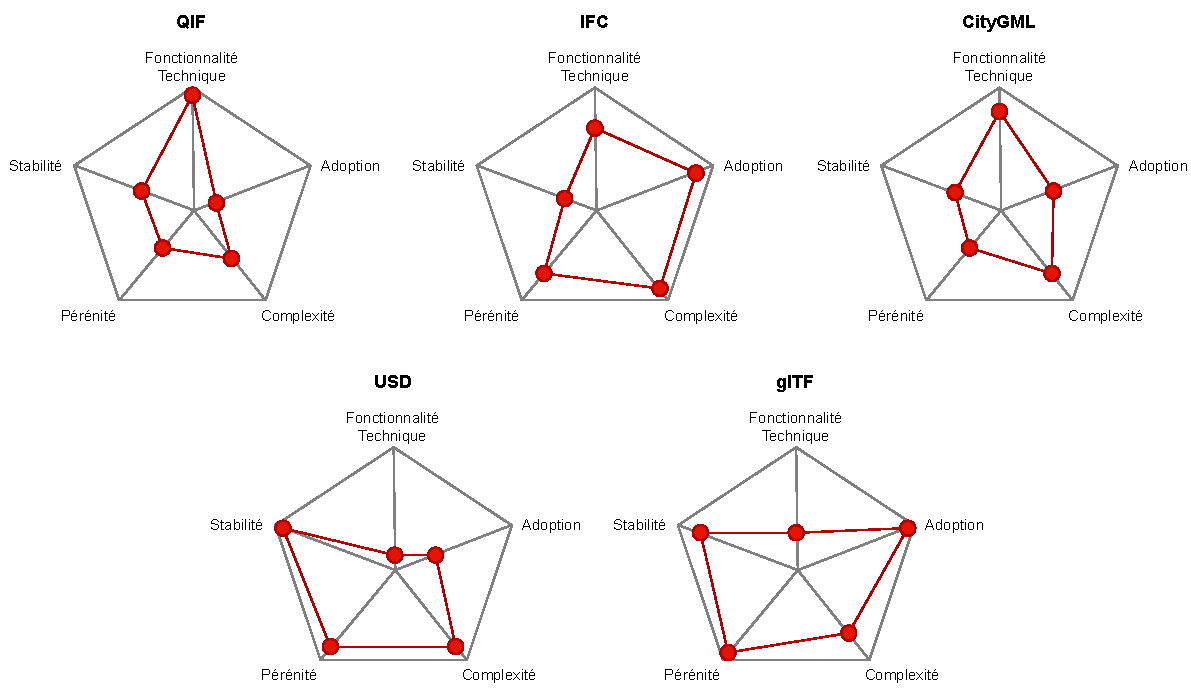
\includegraphics[width=1\linewidth]{imports/3DFiles_Evaluation.pdf}
    \caption{Évaluation globale des formats de fichiers}
    \label{fig:enter-label}
\end{figure}

Les formats de fichiers spécifiques à des domaines d'études tel que le gbXML pour les études énergétiques, le SAF pour l'analyse structurel ou encore l'ILCD pour l'analyse de cycle de vie n'ont pas été étudiés. Cela mériterait une étude complète sur le rapprochement sémantique des différents formats et standards. 

Cependant, constater la complexité des schémas d'informations et l'impossibilité de créer un standard universel de format de fichier 3D (dû aux divergences d'intérêts des utilisateurs finaux) tend à renverser la problématique.

Faut-il nécessairement recourir à l'emploi d'un fichier pour transmettre un ensemble d'information d'un programme à un autre ?
Les containers d'informations sont-ils les seuls à offrir la capacité d'échanger des données entres utilisateurs ?

J'estime qu'il serait plus pertinent de mettre à plat l'ensemble des travaux réalisés par les différentes communautés et consortiums, établir un schéma de donnée évolutif au cas d'usage et le porté sur une technologie conçue spécifiquement pour l'échange d'information à très haute performance : la base de données.

Les systèmes tels que PostgreSQL, MongoDB et autres sont justement prévus pour accueillir un volume considérable d'information. Ils disposent également de toutes les technologies nécessaires au partage de ces données à très haut débit, voir en temps réel, à un ensemble d'utilisateurs. Les API (REST et autres) permettent l'interropérabilité d'à peu près n'importe quel système d'information et application avec des systèmes de gestion de base de données.

Ces technologies sont, par ailleurs, parfaitement compatibles et largement déployés sur le web.


\medskip






%===================================================================

\newpage
\pagestyle{fancy}
\lhead{}
\chead{}
\rhead{}
\lfoot{\projecttitle}
\cfoot{}
\rfoot{}

\bibliographystyle{IEEEtran}

\bibliography{imports/bibliography} 


\end{document}
%==[DO NOT CHANGE ANYTHING HERE]====================


